\subsection{CPU, Scheduling, and OS Services}

\subsubsection{Measurement overhead}

\paragraph{Methodology}
As we are microbenchmarking, the overhead of the measurement tools that we
choosed may influence our results. Thus we need to know the cost of reading
the clock and since we are using loops for averaging the results of the tests, we
also need to know the overhead caused by these loops.\\
We are using the \emph{rdtsc} assembly instruction to do the measurement.
The \emph{rdtsc} instruction allows us to read the \emph{Time Stamp Counter}
which is a 64 bit counter containing the number of cycles elapsed since his
reset.\\
In terms of implementation, the instruction is integrated in the code using
inline assembly and is called using a function which is inlined to avoid the
overhead of the procedure call and the stack frame creation.
To measure the cost of the reading clock operation, we measured the result between
two calls and repeated the operation 100,000 times.\\
The loop overhead has been measured with 100,000 iterations.

\paragraph{Predictions}
The operations between the two rdtsc call are basicly a copy from the result
which are stored in the eax and edx register to the main memory, a binary shift
and a binary OR on the two variables.
As the cache may be hited, it's basicly two cache write, around 10 cycles, and
the cost of the second rdtsc call.\\

As the loop optimization is turned on, the cost of a loop iteration is basicly a
an incrementation in a register, a comparaison and a jump.
The total cost may be around 3 cycles if we count 1 cycle per operation such as
incremention, comparaison and jump.\\

There is no software overhead in any of these operations.

\paragraph{Results}
\begin{table}[h]
\begin{center}
\begin{tabular}{| l | l | l | l | l |} \hline
Operation 			& Hardware cost 	& Software cost 	& Prediction	& Measured \\ \hline
Reading the clock 	& 25 cycles		& 0 cycles			& 25 cycles 	& 58.555 cycles \\ \hline
Loop 				& 2 cycles 		& 0 cycles & 2 cycles 	& 0.517 cycles \\ \hline
\end{tabular}
\end{center}
\caption{Measurement overhead\label{tab:measurement-overhead}}

\end{table}

As seen in table \ref{tab:measurement-overhead}, our estimates are too low for the reading time compared to the actual result.
The reason may be that the cost of the memory write operation is higher than excepted.
It seems that we feel the cache latency due to the dependency of the data avoiding the effective use of the pipelining.
This hypothesis on the memory write operation cost is due to the fact that on long run,
the result is lowered to aproximatly 30 cycles after 50,000 iterations.
We choosed to report the average of a run which did not show this reduction in
the cost because it seems more accurate (i.e. we will call rdtsc once for each
loop).\\

Our estimates are in the good range for the loop.

\paragraph{Success of Methodology}
Our result for the reading time of the clock are varying but we have a good average result.
As the overhead will be accounted only once for many iterations, this will not
cause more problem.\\

The result for the loop overhead seems accurate and the optimizations seem
efficient.

\subsubsection{Procedure call overhead}
\paragraph{Methodology}
We defined seven functions with different number of arguments to test the
cost of a procedure call and the overhead of an argument.
Each procedure call is made 100,000 time in a loop and the total is measured.
The cost per loop cycle is then calculated and the overhead of the loop is
removed.

\paragraph{Predictions}
On x86-64 a procedure call is composed off :
\begin{enumerate}
\item Moving the arguments into specific registers (for the 7 first arguments)
\item Calling the procedure, that is jumping to the beginning of the procedure
\item Creating a new stack frame, that is saving the previous stack pointer and
moving the stack pointer into the begin stack pointer
\item Destroying the stack frame
\item Restoring the instruction pointer
\end{enumerate}

The latency of the memory operations may be hidden due to pipelining.
The procedure call should normally be predicted by the branch prediction part of
the processor avoiding stall of the processor.
The architecture of the Intel Sandy Bridge is very complex, making prediction is
really difficult.
We can guess that the procedure call will take about 10 cycles and that each
argument will cause a cost of one cycle due to the new register access.

\paragraph{Results}
\begin{table}[h]

\begin{center}
\begin{tabular}{| l | l | l | l | l |}
\hline
\# of args 	& Hardware cost 	& Software cost & Prediction & Measured \\ \hline
0 & 2 cycles 	& 8 cycles  		& 10 cycles 	& 14.471 cycles \\ \hline
1 & 2 cycles 	& 9 cycles  		& 11 cycles 	& 14.471 cycles \\ \hline
2 & 2 cycles 	& 10 cycles  		& 12 cycles 	& 14.455 cycles \\ \hline
3 & 2 cycles 	& 11 cycles 		& 13 cycles 	& 14.462 cycles \\ \hline
4 & 2 cycles 	& 12 cycles 		& 14 cycles 	& 14.461 cycles \\ \hline
5 & 2 cycles 	& 13 cycles 		& 15 cycles 	& 14.461 cycles \\ \hline
6 & 2 cycles 	& 14 cycles 		& 16 cycles 	& 14.456 cycles \\ \hline
7 & 2 cycles 	& 15 cycles 		& 17 cycles 	& 16.518 cycles \\ \hline
\end{tabular} \\
\end{center}
\caption{Procedure calls\label{tab:procCall}}
\end{table}
\begin{figure}[h]

\begin{center}
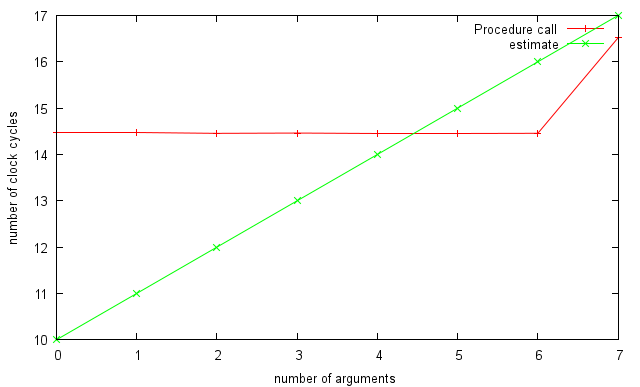
\includegraphics[scale=0.8]{procCallImage}
\end{center}
\caption{Procedure calls\label{fig:procCallf}}
\end{figure}

As what we can see in figure \ref{fig:procCallf} and table \ref{tab:procCall}, the results are low as predicted.
Apparently the cost of accessing one more register is too low to be detected.
The result is changing only when the function take 7 aguments, because the last
one is not put into a register.
The 7th argument is put into the stack and the cost for doing that turns out to
be about 2 cycles (cache hit).

\paragraph{Success of Methodology}
The methodology we used for testing procedure call is quite successful.

At first, we tried to use a function which sums up the parameters it takes to
avoid compiler optimization.
As a result, the running time for procedures gave different number dependent of
the number of arguments.
However, this is mainly due to the number of add operations which preformed in that case.
We then found a trick (using \emph{asm("");}) to avoid compiler optimization.

At the beginning we also had a result increasing due to the fact that gcc was
compiling in 32 bits mode.
In 32 bits, the calling convention is different and the arguments are passed
through the stack.
Afterall, we got result shown in figure \ref{fig:procCallf}.
At first we were really confused about it, later we realized that not all of
the arguments are put on to the stack on x86-64 CPUs.




\subsubsection{System call overhead}
\paragraph{Methodology}
We choosed the getpid() system call to test the overhead for a minimal system
call as it's supposed to be the least expensive system call.
We then ran it 10,000 times to get an averaged result.

\paragraph{Predictions}
System call are expected to be more expensive than simple procedure call as they
produce a context switch.
The state of the process need to be saved and a kernel thread must be launched.
The way back need also to be done.
We except something like 400 cycles for each context switch, so a total of about 800 cycles.

\paragraph{Results}
\begin{table} [h]
\begin{center}
\begin{tabular}{| l | l | l | l | l |}
\hline
Operation 				& Hardware cost & Software cost & Prediction & Measured \\
\hline
Context switch (1st run) & 200 cycles & 600 cycles & 800 cycles & 5000 cycles\\
\hline
Context switch (average) & 200 cycles & 600 cycles & 800 cycles & 750 cycles\\
\hline
\end{tabular}
\end{center}

\caption{System calls\label {tab:sysCall}}
\end{table}


As what we can see in table \ref{tab:sysCall}, the first call is always slow,
due to the need to read kernel code and kernel memory which are not in cache.
As we discussed ealier, the fact we are using virtual machine is giving us worse
performances on TLB misses.
The first system call may experience a TLB miss.
The following calls are going faster probably due to branch prediction and
cache.

\paragraph{Success of Methodology}
We can see that system calls are much expensiver than procedure calls as excepted.
First of all, system call by itself is a normal procedure call, it need to do everything a procedure call need to do.
Secondly, the system call need more time for loading function and switching to the kernel mode.
The way we did our measurement seems to be successful.



\subsubsection{Task creation time}
\paragraph{Methodology}
We measured the time to create process and thread seperately and
compared the results to verify our measurement.

For thread and process creation we waited until the newly created thread/process
finishes for each measurement.
We did this because otherwise the kernel could be lazy and create part of
the information later.
Thus our measurement include two context switches and one other syscall.
We used the system call fork() to create a new process.
The number of cycles is recorded before the fork() is called and after the waitid()
returns meaning that the new process has exited.
For the newly created process, we called \_exit() to immediately exit after creation.

Similarly, for the thread, we used the native solaris implementation,
which is thr\_create() to create threads.
At first we used the pthread library for thread creation operation.
We replaced it with thr\_create() later because it is not a native Solaris
implementation, which is not as accurate when we are doing the measurement
of the whole Solaris OS.
Right after the creation of the thread, we used thr\_join() to wait for the
termination of the new created thread.

We also measured the time for the program to create the first process and the
first threads.
It shows the time needed to load the functions we used in this measurement into the cache.

The creation overhead has been measured with 100,000 iterations.

\paragraph{Predictions}

When a new process is created, all the page table entries of the process virtual
memory need to be copied.
On a new process creation, the kernel needs also to duplicate the information
regarding the open files and other kernel tables.

When we create a kernel thread, less information are copied because all the
resources of a thread except the stack are shared with the main thread.

As mentioned earlier, the thread has less data to copy than process do.

We think that process creation may take about 15000 cycles and that a thread
creation may take 10000 cycles.


\paragraph{Results}
\begin{table}[h]
\begin{center}
\begin{tabular}{| l | l | l | l | l | l |}
\hline
Operation & H/W cost & S/W cost & Prediction & Measured average & Measured first creation \\
\hline
fork() process 		& 5000 cycles & 10000 cycles 	& 15000 cycles& 1198519.65 cycles & 2257852 cycles\\ \hline
thr\_create() thread 	& 100 cycles & 99000 cycles	& 10000 cycles &
157433.27 cycles & 2233593 cycles\\ \hline
\end{tabular}
\end{center}
\caption{Task creation time\label{tab:task-creation}}

\end{table}

As seen in table \ref{tab:task-creation}, the measurement result mostly fits our prediction besides the fact that the number of cycles are way bigger than what we expected.
This difference is probably cause by the cost of the memory operations

\paragraph{Success of Methodology}
One problem with our methodoly is that it includes creation and destruction of
the process/thread.
This idea is actually comming from the lmbench paper and it seems to make sense.
Our result successfully show the cost of creating a new process instead of a
thread.


\subsubsection{Context switch time}
\paragraph{Methodology}

We measured the context switching time for both processes and threads.
The methodology originally comes from the paper \emph{lmbench: Portable Tools for Performance
Analysis}.
We used pipes in order to measure these values.
However, pipes creates an overhead by themself.
We measured the pipe overhead seperately.
As the other thread/process is waiting to read, writting into the pipe is
forcing a context switch to kernel mode and allow the kernel to unlock the
waiting process.
We only wrote an integer to avoid increasing the overhead.

Similar to the previous task creation measurement, we used fork() and
thr\_create() to create new process and threads.
The threads/processes are arranged into a circle created with pipes.
Each thread/process is doing a blocking read on a pipe connected to the previous
thread and a write on a pipe connected to next thread in an infinite loop.
The thread/process is composed of 20 pipes/processes/thred.

The measurement is run 10,000 times to average the result.
The overhead of the pipe is removed in the final result.

\paragraph{Predictions}
%FIXME
Based on the previous results, we can define an upper bound for the cost of a
context switch which is half of the cost of a creation of the task type.
Similar to task creation time, we would expect to see a smaller cost
for the thread context switching than for process context switching as the virtual
address space doesn't need to be changed.
Based on the task creation time we can see in table \ref{tab:task-creation},
our prediction for process context switching is 200,000 clock
cycles and for process context switching is 75,000 clock cycles.

Meanwhile, our prediction for the pipe overhead is 1000 clock cycles per syscall
on the pipe.
We base this estimation on the cost of a minimal syscall and we add an overhead
for the complexity of the pipe.

\paragraph{Results}
\begin{table}
\begin{center}
\begin{tabular}{| l | l | l | l | l |}
\hline
Operation 		& Hardware cost 	& Software cost 	& Prediction 	& Measured \\ \hline
Process context switch 	& 		& 	&2000000 cycles	& 100540.28 cycles \\ \hline
Thread context switch 	& 		&		&1500000 cycles	& 94764.77 cycles \\ \hline
Pipe overhead		& 		&		&30000 cycles	& 45275.283 cycles \\ \hline
\hline
\end{tabular}
\end{center}

\caption{Context switch time\label{tab:context-switch-time}}
\end{table}
As what we can see in table \ref{tab:context-switch-time}, same as what we expected, the time it takes for context switching between threads is a lot shorter than the one for processes.

\paragraph{Success of Methodology}
We measured the context switching overhead for both processes and threads. The overhead of such context switching is going to be the time start from the creation of the child to the time execution gets back to the parent process/thread excluding the time for child to execute. We only tested the context switching within 2 different processes. Due to the lack of time, we were not measuring the context switching time among more than 2 processes. However, this is something good to measure in a real situation because it makes more sense to execute the program using the optimized number of threads in order to get ebst performance.



